%% chapters/chapter_2.tex
%%
%% Copyright 2017 Evandro Coan
%% Copyright 2012-2014 by abnTeX2 group at http://abntex2.googlecode.com/
%%
%% This work may be distributed and/or modified under the
%% conditions of the LaTeX Project Public License, either version 1.3
%% of this license or (at your option) any later version.
%% The latest version of this license is in
%%   http://www.latex-project.org/lppl.txt
%% and version 1.3 or later is part of all distributions of LaTeX
%% version 2005/12/01 or later.
%%
%% This work has the LPPL maintenance status `maintained'.
%%
%% The Current Maintainer of this work is the Evandro Coan.
%%
%% The last Maintainer of this work was the abnTeX2 team, led
%% by Lauro César Araujo. Further information are available on
%% https://www.abntex.net.br/
%%
%% This work consists of a bunch of files. But originally there were 2 files
%% which are renamed as follows:
%% Deleted the `abntex2-modelo-img-marca.pdf`
%% Renamed the `abntex2-modelo-include-comandos.tex, v-1.9.2 laurocesar` to `chapters/chapter_1.tex`
%%
% ---
% Este capítulo, utilizado por diferentes exemplos do abnTeX2, ilustra o uso de
% comandos do abnTeX2 e de LaTeX.
% ---

% The \phantomsection command is needed to create a link to a place in the document that is not a
% figure, equation, table, section, subsection, chapter, etc.
% https://tex.stackexchange.com/questions/44088/when-do-i-need-to-invoke-phantomsection
\phantomsection

% https://tex.stackexchange.com/questions/5076/is-it-possible-to-keep-my-translation-together-with-original-text
\chapter{Deep Learning}\label{chap:deep-learning}

The advent of deep learning has revolutionized several fields, offering unprecedented capabilities in pattern recognition, decision-making, and problem-solving~\cite{Goodfellow-et-al-2016}.
In the realm of combinatorial optimization, particularly MILP, traditional methods often encounter computational bottlenecks when solving large-scale instances.
However, recent strides in deep learning have opened up exciting avenues for developing effective primal heuristics.
This chapter delves into the background of deep learning, focusing on the fundamental principles of supervised learning and neural network architectures.
The understanding of such concepts is essential for exploring the design and implementation of deep-learning-based solution prediction models tailored to MILP instances.


\section{Supervised Learning}

Supervised learning can be seen as the problem of finding a function that best associates inputs $x$ to outputs $y$ given a \emph{training set} with finitely many examples of such inputs and outputs~\cite{Goodfellow-et-al-2016}.
Although the machine learning (ML) area has attracted plenty of attention in the last decade, this learning problem is not new.
In fact, the core concepts were already established in the 1960s and 1970s~\cite{vapnikNatureStatisticalLearning2000}.
This section's approach to supervised learning will be that of statistical learning theory, based on \citeonline{vapnikNatureStatisticalLearning2000}, but with a more modern notation, derived from pattern recognition~\cite{bishopPatternRecognitionMachine2006,hastieElementsStatisticalLearning2009}.

\subsection{Supervised learning algorithm}

Supervised learning will be defined here as a problem of estimating a function that minimizes the risk.
Let $\mathcal{X}$ and $\mathcal{Y}$ be the input and output space, and $\mathcal{P}$ be a joint probability distribution~\footnote{Or a joint probability density function, in the case of continuous spaces.} over $\mathcal{X}\times \mathcal{Y}$.
To evaluate a function $f: \mathcal{X} \longrightarrow \mathcal{Y}$ with respect to its capacity to perform the correct association between an input $x\in \mathcal{X}$ and an output $y\in \mathcal{Y}$, one measure's the discrepancy, or the \emph{loss}, $\ell(y,f(x))$.
In this context, the \emph{risk} associated to $f$ over the joint distribution $\mathcal{P}$ is the expected value of the loss function, or \[
    R(\mathcal{P},f) = \int_{\mathcal{X}\times \mathcal{Y}} \ell(y,f(x))\mathcal{P}(x,y)
    %R(f) = \mathbb{E}_{(x,y)\sim \mathcal{P}} \ell(y,f(x))
.\] 

% \color{red}
  % [COMMENT: I didn't quite understand the definition  above. Let $x$ and $y$ be two continuous random variables with a joint density function $g(x,y)$. Then wouldn't the expected value of the loss function be $\int_{X\times Y} \ell(y,f(x))\cdot g(x,y)\cdot dx\cdot dy$?]
% \color{black}

The machine learning paradigm is that the joint probability function is fixed but unknown, and one only has access to a finite number of samples~\cite{vapnikNatureStatisticalLearning2000}.
This idea is best represented through a \emph{dataset}, which is a finite set $\mathcal{D}$ of independent and identically distributed (i.i.d.) samples drawn according to $\mathcal{P}$.
In this context, the \emph{empirical risk} associated to a function $f$ over a dataset $\mathcal{D}$ is \[
    R_\textrm{emp}(\mathcal{D},f) = \frac{1}{|\mathcal{D}|} \sum_{(x,y)\in \mathcal{D}} \ell(y, f(x))
.\]

In this work, it is considered that the function to be estimated is chosen from a \emph{parametric model}\footnotemark, which is a family of functions $f_\theta: \mathcal{X} \longrightarrow \mathcal{Y}$ defined over a parameter space $\Theta \ni \theta$.
\footnotetext{This is in contrast to non-parametric models, whose functions' parameters are defined in terms of the dataset~\cite{murphyMachineLearningProbabilistic2013}.}
The problem then becomes that of finding a parameter vector that minimizes the empirical risk from a dataset $\mathcal{D}$, or \emph{fitting} a model to a dataset, denoted
\begin{equation}\label{eq:cost-minimization}
    \min_{\theta \in  \Theta} \mathcal{L}(\theta)
,\end{equation}
where
\begin{equation}\label{eq:cost-function}
    \mathcal{L}(\theta) = \frac{1}{|\mathcal{D}|} \sum_{(x,y)\in \mathcal{D}} \ell(y, f_\theta(x))
\end{equation}
is an alternate, commonly found notation for the empirical risk, which often carries the name \emph{cost function}~\cite{murphyMachineLearningProbabilistic2013,Goodfellow-et-al-2016}.
Both ``empirical risk'' and ``cost function'' will be used interchangeably throughout this dissertation, although the former has a stronger connection to learning theory, while the latter is more related to practical matters.

A supervised learning algorithm is essentially an algorithm to optimize a cost function given a model and a dataset.
In fact, it is possible to define a supervised learning algorithm as a simple recipe: ``combine a specification of a dataset, a cost function, an optimization procedure and a model''~\cite{Goodfellow-et-al-2016}.
Many different algorithms exist that are suitable for different components of this recipe.
\textcolor{blue}{For example, there are algorithms which are tailored for the synthesis of decision-tree models~\cite{breimanClassificationRegressionTrees2017}.}
The least squares algorithm (used in the example of Section~\ref{sec:generalization-overfitting}) can be seen as a supervised learning algorithm for polynomial models and the squared error loss function.


%%%%%%%%%%%%%%%%%%%%%%%
\subsection{Generalization and overfitting}\label{sec:generalization-overfitting}

Blindly minimizing the empirical risk can lead to a problem named \emph{overfitting}.
Overfitting happens when the empirical risk does not reflect the true risk, that is, when a function is \emph{fit} for the dataset, but not for the underlying data distribution.

This concept is best understood through an example.
Suppose $\mathcal{X},\mathcal{Y}\subseteq\R$ and that a dataset $\mathcal{D}$ with 40 i.i.d. samples is obtained such as illustrated in Fig.~\ref{fig:overfitting-example}.
It is desired to find a function that minimizes the risk measured through the squared error loss \[
    \ell(y,f(x)) = (y-f(x))^2
.\] 
The models $f^{(1)},f^{(2)},f^{(3)}$ are polynomials of degree 1, 3, and 15, whose parameters are the weights of the polynomials.
These models are adjusted using least squares algorithm, resulting in parameter vectors $\theta_1^*,\theta_2^*,\theta_3^*$ that achieve a global minimum of the empirical risk with their respective models.
The performance of these models is illustrated in Fig.~\ref{fig:overfitting-example}.

Note that model $f^{(3)}$ achieves the lowest empirical risk on $\mathcal{D}$.
However, $f^{(2)}$ is the one that seems to best associate inputs to outputs, considering a visual intuition of the underlying data distribution.
One could say that $f^{(3)}$ is \emph{too complex} for the underlying distribution, which leads to it being more tightly adjusted to the noise present in the dataset rather than on the underlying data distribution~\cite{murphyMachineLearningProbabilistic2013}.
On the other hand of the spectrum is the $f^{(1)}$ model, which is not complex enough to model the desired behavior.
While $f^{(3)}$ is overfitting the data, $f^{(1)}$ is underfitting it.

\begin{figure}[h]
    \centering
    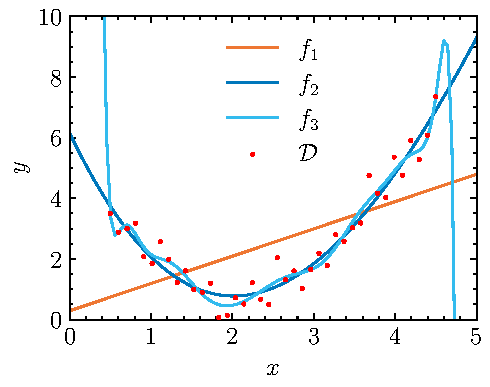
\includegraphics{pictures/overfitting.pdf}
    \caption{Example of overfitting. The three models shown ($f^{(1)},f^{(2)},f^{(3)}$) are families of polynomials of degree 1, 3 and 15, respectively. The optimal parameter vectors $\theta_1^*,\theta_2^*$ and $\theta_3^*$ were optimized to the dataset $\mathcal{D}$ using a the least squares algorithm. The empirical risks are $\mathcal{L}(\theta_1^*)=79.67$, $\mathcal{L}(\theta_2^*)=7.64$, and $\mathcal{L}(\theta_3^*)=5.48$.}
    \label{fig:overfitting-example}
\end{figure}

The level of overfitting that a function $f$ presents could be determined through the \emph{generalization gap}, which is the difference between the empirical risk and the true risk $R(\mathcal{P},f) - R_\textrm{emp}(\mathcal{D},f)$~\cite{murphyMachineLearningProbabilistic2013}.
More specifically, a function can be said to overfit the dataset if it has a high generalization gap.
As the underlying distribution $\mathcal{P}$ is not known, the generalization gap is approximated by \emph{splitting} the dataset $\mathcal{D}$ into a training set $\mathcal{D}_\textrm{train}$ and a test set $\mathcal{D}_\textrm{test}$.
The idea is that the parameters of the model are adjusted according to the empirical risk of $\mathcal{D}_\textrm{train}$, while $\mathcal{D}_\textrm{test}$ is reserved for estimating the true risk, also called \emph{generalization error}.
This way, the resulting function cannot be overfitted to $\mathcal{D}_\textrm{test}$, which is kept as an untouched source of information of the underlying distribution.
Finally, the generalization gap can be estimated as  \[
    R_\textrm{emp}(\mathcal{D}_\textrm{test},f) - R_\textrm{emp}(\mathcal{D}_\textrm{train},f)
.\] 

\subsection{Hyperparameter tuning}

Hyperparameters are the settings that modify the behavior of a supervised learning algorithm~\cite{Goodfellow-et-al-2016}.
These hyperparameters can be configurations of the optimization algorithm or parameters of the model that are not adjusted by the algorithm.
Hyperparameter adjustment is impactful both in the runtime of the algorithm and in the quality of the function returned.

In the polynomial fitting example above (illustrated in Fig.~\ref{fig:overfitting-example}), the polynomial degree is a hyperparameter.
Different values for this hyperparameter result in totally different parameter spaces $\Theta$ over which the optimizer will search for a risk minimizer.
If a ridge regression algorithm is used instead of the least squares to find the optimal function, then a hyperparameter is the weight of the $\ell_2$-norm of $\theta$.
Such hyperparameter does not alter the function space associated with $\Theta$ but guides the optimizer towards different optima.

Given the impact of the hyperparameters in the function space, another way of looking at hyperparameters is as a means to encode prior beliefs of the underlying data distribution~\cite{murphyMachineLearningProbabilistic2013}.
Again on the polynomial fitting example, if one believes that the outputs are approximately related to the inputs through a 5-th degree polynomial, then this information can be directly encoded in the hyperparameters of the algorithm.
Another example is the belief that the output has a seasonal component with respect to a given input, which could be used to restrict the parameter space to periodic functions.

Unfortunately, and mainly for complex, high-dimensional spaces, the existence of strong and sufficient prior beliefs is rarely assumed in supervised learning problems.
On the contrary, the tuning, or optimization, of hyperparameters is a common step in machine learning projects.
A new hold-out set is necessary to compare different choices of hyperparameter values.
This is because hyperparameters that control model capacity are always biased towards greater capacity~\cite{Goodfellow-et-al-2016}.
In other words, if the impact of different hyperparameter values is evaluated on the training dataset $\mathcal{D}_\textrm{train}$, it will likely lead to choosing the value that implies a greater model capacity, which leads to overfitting.
As it is assumed that the test dataset $\mathcal{D}_\textrm{test}$ is not available during training to avoid a biased estimation of the generalization error~\cite{murphyMachineLearningProbabilistic2013}, a second held-out set is necessary.

In practice, the available data $\mathcal{D}$ is partitioned into three disjoint sets:
\begin{itemize}
    \item[$\mathcal{D}_\textrm{train}$] the training set, which is used for fitting the model, i.e., the best parameter vector $\theta^*$ is chosen such that the cost function over $\mathcal{D}_\textrm{train}$ is minimized;
    
    \item[$\mathcal{D}_\textrm{val}$] the validation set, which is used to measure the impact of different values for the hyperparameters; and
    
    \item[$\mathcal{D}_\textrm{test}$] the test set, which is used to estimate the generalization error (empirical risk) of the function returned by the supervised learning algorithm with the best hyperparameter values found.
\end{itemize}
A usual ratio is to set apart 50\% of the samples in $\mathcal{D}$ for the training set, 25\% for the validation set, and 25\% for the test set~\cite{hastieElementsStatisticalLearning2009}.


%%%%%%%%%%%%%%%%%%%%%%%%%%%%%%%%%%%%%%%%%
\section{Deep Neural Networks}

Deep feedforward neural networks ``are the quintessential deep learning models''~\cite{Goodfellow-et-al-2016}.
Feedforward neural networks (NNs) are compositions of differentiable functions such that the information flows without any sort of feedback connection.
An NN model can be written as
\begin{align*}
    f_\theta: \R^{n} &\longrightarrow \R^{m} \\
    x &\longmapsto f_\theta(x) = f^{(L)}_\theta(f^{(L-1)}_\theta(\cdots(f^{(1)}_\theta(x))\cdots))
,\end{align*}
in which each $f^{(l)}_\theta$, $l=1,\ldots,L$, is a \emph{layer} of the network, and $L$, the number of layers.
All layers except the last one are called \emph{hidden} layers of the network.
The last one is called the \emph{output} layer.
A simple layer of an NN can be a linear combination of its inputs followed by a nonlinear function $\sigma : \R^{d} \longrightarrow \R^{d}$, as in \[
f^{(l)}_\theta = \sigma\left( W^{(l)} x + c^{(l)} \right) 
.\] 
Note that an NN's parameter vector can be seen as the concatenation of the parameters of all layers, i.e., $\theta = (W^{(1)},c^{(1)},W^{(2)},c^{(2)},\ldots,W^{(L)},c^{(L)})$.
In the hidden layers, the default choice for $\sigma$, the \emph{activation function}, is the rectified linear unit, or ReLU~\cite{Goodfellow-et-al-2016}, defined element-wise as $\sigma(z)=\max\{0,z\}$.
The activation function of the output layer is application-dependent.

% The number of layers, or \emph{depth}, of NNs is what characterizes deep learning.
% While traditional machine learning models require substantial manual engineering effort to generate features that are able to provide to ML models sufficient, and high-quality information

Deep neural networks (DNNs) are a larger family of models.
Although DNNs are also composed of differentiable functions, these functions are assembled in any form of directed acyclic graphs~\cite{murphyMachineLearningProbabilistic2013}.
Note that this opens up complex architectures that may contain feedback, memory, convolutions, etc.~\cite {Goodfellow-et-al-2016}.

\subsection{Gradient-based learning}

% See Bengio et al., Ch. 6.2
Because of the inherent nonlinearities of NNs, the cost (or empirical risk) minimization problem \eqref{eq:cost-minimization} becomes nonconvex under the most common loss functions~\cite{Goodfellow-et-al-2016}.
As NNs are, by definition, differentiable, they are usually trained by using gradient-based optimizers.
The gradient-descent method is one of the oldest algorithms for finding local minima of a function~\cite{cauchy1847}.
Such algorithms take successive steps of the form
\begin{equation}\label{eq:grad-step}
    \theta \gets \theta - \lambda\, \nabla \mathcal{L}(\theta)
,\end{equation}
such that with a sufficiently small \emph{learning rate} $\lambda>0$, the parameter vector is always modified such that the cost function is minimized.

A practical problem of gradient descent is that large training sets are often necessary to achieve low generalization errors, which, in turn, increases the computational cost of calculating the gradient.
A solution is to break down the parameter vector update step \eqref{eq:grad-step} stochastically in an algorithm called stochastic gradient descent (SGD).
This is intuitively sound because the gradient of the empirical risk is already an expectation of the gradient of the actual risk. 
Thus, instead of approximating the gradient using the entire training dataset, it is possible to approximate the gradient by sampling a limited number of examples from it.
In other words, instead of computing the gradient as \[
    g = \nabla \mathcal{L}(\theta) \gets \frac{1}{|\mathcal{D}_\textrm{train}|}\sum_{(x,y)\in \mathcal{D}_\textrm{train}} \nabla_\theta \ell(y,f_\theta(x))
,\] in SGD it is computed as \[
\widetilde{g} \gets \frac{1}{|\mathcal{B}|}\sum_{(x,y)\in \mathcal{B}} \nabla_\theta \ell(y,f_\theta(x)) 
,\] where $\mathcal{B}\subset \mathcal{D}_\textrm{train}$ such that $|\mathcal{B}|\ll |\mathcal{D}_\textrm{train}|$, and then update the parameter vector as \[
\theta \gets \theta -\lambda\, \widetilde{g}
.\] 
The set $\mathcal{B}$ is called a \emph{minibatch} and it is usually sampled uniformly from the training set~\cite{Goodfellow-et-al-2016}.

Although gradient descent can provide convergence guarantees to local optima of nonconvex functions under mild conditions, it has been regarded as a slow and unreliable optimization method.
However, deep learning applications stand out, as it has been empirically shown that SGD is a reliable method to achieving sufficiently small cost function values~\cite{Goodfellow-et-al-2016}.
Arguably, this can be traced back to the generalization problem.
Differently from the traditional optimization paradigm, in which the performance is evaluated on the function being optimized, a learning algorithm optimizes indirectly, i.e., the performance metric of interest (generalization error) is not directly optimized.
Therefore, achieving local or global optima is not as relevant for machine learning as it is for the field of optimization.
In fact, local optima can be a source of overfitted parameter vectors.

% Nevertheless, SGD has several shortcomings, which have been addressed plentifully over the last decades.
A prominent problem of SGD is that it can become very slow in face of flat regions, saddle points, and noisy gradients, all of which are abundant in deep learning~\cite{goodfellowQualitativelyCharacterizingNeural2015,Goodfellow-et-al-2016}.
To counter-act such effects, one can add a \emph{momentum} to the computation of the gradient estimate, akin to the physical intuition~\cite{nesterovMethodSolvingConvex1983,polyakAccelerationStochasticApproximation1992}.
Another approach is to use an \emph{adaptive learning rate}, which is dynamically adjusted based on the values of the computed gradient~\cite{jacobsIncreasedRatesConvergence1988}.
The Adam optimizer~\cite{kingma2014adam} combines both momentum and adaptive learning rates, with its name actually deriving from ``adaptive moments.''


%%%%%%%%%%%%%%%%%%%%%%%%%%%%%%%%%%%%%
\subsection{Graph Neural Networks}

% Graphs are a widely used data structure, but their ingestion by neural networks is non-trivial.
% NNs usually take real-valued vectors as inputs, so a naïve approach would be to find a vector encoding of a graph and feed such encoding to the model.
% If there exists a limit to the number of edges of the graphs that constitute the domain of the model, a straightforward encoding could be through the adjacency matrix.

Graph Neural Networks (GNNs) are a particular kind of DNN that is optimized for taking graphs as inputs~\cite{sanchez-lengelingGentleIntroductionGraph2021}.
Note that this is not trivial.
For example, NNs are usually defined over real-valued vector spaces, which would require a vector encoding of a graph to be able to represent them.
Such an encoding could be achieved through the adjacency matrix, but that would not account for graph symmetries, as distinct adjacency matrices can represent the same graph\footnote{In fact, any permutation (row- or column-wise) of an adjacency matrix results in the same graph}.

\color{red}
COMMENTS:
\begin{itemize}
\item GNN is a pivotal concept of your research and dissertation. Being abstract, the introduction of a concrete, illustrative GNN would greatly help the reader to understand. The features and operators could be concretely illustrated in the example.

\item The understanding of GNN will also benefit its application in primal heuristics.
\end{itemize}
\color{black}

A GNN takes as input a graph with feature vectors associated to each node.
GNNs are also feedforward networks, i.e., they can be represented by a stacking of layers.
Each layer of the GNN works by propagating feature information between neighboring nodes, which can be seen as \emph{message-passing}~\cite{gilmerNeuralMessagePassing2017}.
More specifically, a layer computes messages that each node emits to its neighbors based on their feature vectors.
Then, each node's output feature vector is computed based on the input feature vector and the messages emitted by the node neighbors.
% Each node's features along with the messages emitted by its neighbors is the information used to compute the feature vector associated to that node in the layer's output graph.
% The feature update can also be seen as a graph \emph{convolution} due to its similarities to the operations in convolutional neural networks~\cite{daigavaneUnderstandingConvolutionsGraphs2021}.

Let $G=(V,E)$ be a graph, $H =\left\{ h_v\in \R^{d}: v\in V \right\} $ be an associated set of node feature vectors, and $f_\theta = f_\theta^{(L)} \circ \cdots \circ f_\theta^{(1)}$ be a GNN with $L$ layers.
Each layer of the GNN has two major components: a message function $M(\cdot)$ and an update function $U(\cdot)$.
The message function computes the messages emitted by each node, while the update function feeds on these messages to update each node's feature vector.
Putting it into terms, each layer $f^{(l)}_\theta$, $l=1,\ldots,L$, of the GNN transforms the previous layer's feature vectors $H^{(l-1)}=\left\{ h^{(l-1)}_v : v \in V \right\}$ through 
\[
% Eduardo Camponogara: Will each layer (l) have an entry (neuron) for each "v"? Does it mean that a  node "v" appears multiple times in the NN, once in each layer?
     h^{(l)}_v = U^{(l)}\left( h^{(l-1)}_v , \left\{ M^{(l)}(h^{(l-1)}_u):u\in \mathcal{N}(v) \right\}  \right) , \forall v \in V
,\] where $\mathcal{N}(v)$ denotes the set of neighbors of $v$.
Note that each layer maps feature vectors into features vectors, i.e., $f_\theta^{(l)}: H^{(l-1)} \mapsto H^{(l)}$.
The structure of the graph is embedded into this computation by the neighbors function $\mathcal{N}(\cdot)$.

As each node can have an arbitrary number of neighbors, it is reasonable for update functions to contain some sort of aggregation, or \emph{pooling}, mechanism, i.e., a way to compute a fixed-size representation of the messages received.
A common choice is to sum all messages element-wise, as each message is a vector of the image of $M^{(l)}$ and, thus, has the same dimension.
Other possibilities are to aggregate through element-wise averaging, maximum, or use some sort of attention mechanism that can be learned along the model parameters~\cite{veličković2018graph}.
Furthermore, a message function can easily be extended to consider edge weights (or even edge features) along with feature vectors of the neighbors.

As an example, let the input space be the set of colored graphs and consider a handcrafted GNN, as illustrated in Fig.~\ref{fig:gnn-example}.
A colored graph will be represented as an undirected graph $G=(V,E)$ paired with a set of node features $H^{(0)}$ such that for each node $v\in V$, there exists a feature vector $h_v^{(0)}\in H^{(0)}$ with an encoding of a color in cyan-magenta-yellow (CMY) format, i.e., $h_v^{(0)}\in [0,1]^3$.
Let $f_\theta$ be a GNN with two layers ($L=2$), such that both layers perform the same operation ($f_\theta^{(1)}=f_\theta^{(2)}$).
The message functions of both layers is the complementarity function, which maps each node's color to its complementary color ($M(h_v) = \bm{1}_3 - h_v$).  
The update functions is a simple average between all messages received.
In summary, the GNN will update each node with the average complementary color of all of its neighbors.

\begin{figure}[h]
    \centering
    \begin{tikzpicture}
	\begin{scope}[local bounding box=l0,every node/.style={circle,draw}]
	    \node[fill={rgb:cyan,1}] (l0n1) at (1,1) {$1$};
	    \node[above right = 1cm of l0n1,fill={rgb:magenta,1}] (l0n2) {$2$};
	    \node[below right = 1cm of l0n1,fill={rgb:yellow,1}] (l0n3) {$3$};
	    \node[below left = 1cm of l0n3,fill={rgb:cyan,0.5;magenta,0.5;yellow,0.5}] (l0n4) {$4$};

	    \path (l0n1) edge (l0n2);
	    \path (l0n2) edge (l0n3);
	    \path (l0n3) edge (l0n4);
	    \path (l0n3) edge (l0n1);
	\end{scope}

	\node[left = 0cm of l0n1] (h0n1) {$h_1^{(0)}=(1,0,0)$};
	\node[left = 0cm of l0n2] (h0n2) {$h_2^{(0)}=(0,1,0)$};
	\node[left = 0cm of l0n3] (h0n3) {$h_3^{(0)}=(0,0,1)$};
	\node[left = 0cm of l0n4] (h0n4) {$h_4^{(0)}=(0.5,0.5,0.5)$};

	\node[fit=(l0n1) (l0n2) (l0n3) (l0n4)] (L0){};

	\begin{scope}[local bounding box=l1,every node/.style={circle,draw}]
	%\begin{scope}[shift={($(l0.east)+(2cm,0)$)},local bounding box=l1,every node/.style={circle,draw}]
	    \node[right = 4 cm of l0n1,fill={rgb:cyan,1;magenta,0.5;yellow,0.5}] (l1n1) {$1$};
	    \node[above right = 1cm of l1n1,fill={rgb:cyan,0.5;magenta,1;yellow,0.5}] (l1n2) {$2$};
	    \node[below right = 1cm of l1n1,fill={rgb:cyan,0.5;magenta,0.5;yellow,0.83}] (l1n3) {$3$};
	    \node[below left = 1cm of l1n3,fill={rgb:cyan,1;magenta,1;yellow,0}] (l1n4) {$4$};

	    \path (l1n1) edge (l1n2);
	    \path (l1n2) edge (l1n3);
	    \path (l1n3) edge (l1n4);
	    \path (l1n3) edge (l1n1);
	\end{scope}

	\node[left = 0cm of l1n1] (h1n1) {$h_1^{(1)}$};
	\node[left = 0cm of l1n2] (h1n2) {$h_2^{(1)}$};
	\node[left = 0cm of l1n3] (h1n3) {$h_3^{(1)}$};
	\node[left = 0cm of l1n4] (h1n4) {$h_4^{(1)}$};

	\node[fit=(l1n1) (l1n2) (l1n3) (l1n4)] (L1){};
	\path [-latex,thick] (L0.north east) edge[bend left] node [above] {$H^{(1)}=f_\theta^{(1)}( H^{(0)} ) $} (L1.north west);

	\begin{scope}[local bounding box=l2,every node/.style={circle,draw}]
	    \node[right = 4cm of l1n1,fill={rgb:cyan,0.5;magenta,0.25;yellow,0.33}] (l2n1) {$1$};
	    \node[above right = 1cm of l2n1,fill={rgb:cyan,0.25;magenta,0.5;yellow,0.33}] (l2n2) {$2$};
	    \node[below right = 1cm of l2n1,fill={rgb:cyan,0.17;magenta,0.17;yellow,0.5}] (l2n3) {$3$};
	    \node[below left = 1cm of l2n3,fill={rgb:cyan,0.5;magenta,0.5;yellow,0.17}] (l2n4) {$4$};

	    \path (l2n1) edge (l2n2);
	    \path (l2n2) edge (l2n3);
	    \path (l2n3) edge (l2n4);
	    \path (l2n3) edge (l2n1);
	\end{scope}

	\node[left = 0cm of l2n1] (h2n1) {$h_1^{(2)}$};
	\node[left = 0cm of l2n2] (h2n2) {$h_2^{(2)}$};
	\node[left = 0cm of l2n3] (h2n3) {$h_3^{(2)}$};
	\node[left = 0cm of l2n4] (h2n4) {$h_4^{(2)}$};

	\node[fit=(l2n1) (l2n2) (l2n3) (l2n4)] (L2){};
	\path [-latex,thick] (L1.north east) edge[bend left] node [above] {$H^{(2)}=f_\theta^{(2)}(H^{(1)})$} (L2.north west);
    \end{tikzpicture}
    \caption{Example of a GNN application to a colored graph. The node features are color in CMY format. Each layer of the model updates the node features with the average complementary color of all of its neighbors.}
    \label{fig:gnn-example}
\end{figure}

\citeonline{kipfSemiSupervisedClassificationGraph2017} have proposed a GNN architecture, in which they use a linear combination of the node features as the messages and weigh them by the number of neighbors of both the emitter and the receiver.
Their update function aggregates the messages by summing them and then feeds the result to a single-layer NN with ReLU activation.
More precisely,
\begin{equation}\label{eq:graph-conv-kipf-2017}
\begin{aligned}
    % M_l(h_u^{(l-1)}) &= \frac{1}{c_{vu}}W^{(l)}h_u^{(l-1)} \\
    % \bm{m}_{u,v}^{(l)} &= \frac{1}{c_{vu}}W^{(l)}\bm{h}_u^{(l-1)},\, u\in \mathcal{N}(v) \\
    h^{(l)}_v &= U^{(l)}\left( h^{(l-1)}_v, \left\{ \frac{1}{c_{v,u}}M^{(l)}(h^{(l-1)}_u):u\in \mathcal{N}(v) \right\}  \right)  \\
    &= \text{ReLU}\left( B^{(l)}h^{(l-1)}_v + W^{(l)} \sum_{u\in \mathcal{N}(v)} \frac{h^{(l-1)}_u }{c_{v,u}} \right)
    % \bm{h}_{v}^{(l)} &= \text{ReLU}\left(\bm{b}^{(l)} + \sum_{u \in \mathcal{N}(v)} \bm{m}_{u,v}^{(l)}\right) \\
    %M^{(l)}(h^{(l-1)}_v) &= W^{(l)}h^{(l-1)}_v
,\end{aligned}
\end{equation}
where $c_{v,u}=\sqrt{|\mathcal{N}(v)|} \sqrt{|\mathcal{N}(u)|} $, and the matrices $W^{(l)}$ and $B^{(l)}$ are trainable parameters of layer $l$~\cite{sanchez-lengelingGentleIntroductionGraph2021}.

Another relevant GNN architecture is the one proposed by \citeonline{hamiltonInductiveRepresentationLearning2017} with the SAGE (SAmple and aGgrEgate) model.
The authors also propose to use a single-layer NN to generate the new feature vectors, but they use the identity as the message function and aggregate them with more complex functions, such as an LSTM (Long Short-Term Memory network).
In such case, the GNN could be written
\begin{equation}\label{eq:graph-sage}
\begin{aligned}
    h^{(l)}_v &= U^{(l)}\left( h^{(l-1)}_v, \left\{ h^{(l-1)}_u:u\in \mathcal{N}(v) \right\}  \right)  \\
    &= \sigma\left( W^{(l)} \left[ \text{LSTM}\left( h^{(l-1)}_u \right)_{u\in \mathcal{N}(v)} , h^{(l-1)}_v \right]   \right)
,\end{aligned}
\end{equation}
where square brackets indicate a vector concatenation~\cite{sanchez-lengelingGentleIntroductionGraph2021}.
Note that the LSTM function could be replaced by any of the aggregation functions the authors propose.



